\section{Durchführung}
\label{sec:Durchführung}
\subsection{Versuchsaufbau}
\label{sub:aufbau}
\begin{figure}[H]
  \centering
  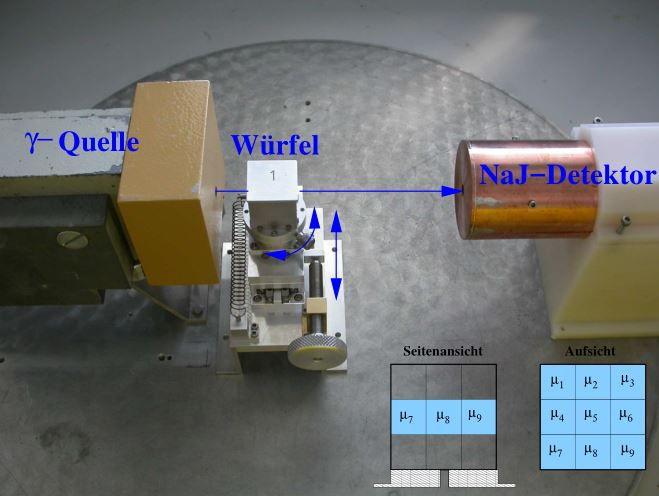
\includegraphics{plots/Aufbau.JPG}
  \caption{Apparatur zur Durchstrahlung der verschiedenen Proben.\cite{Anleitung}}
  \label{fig:Aufbau}
\end{figure}
In Abbildung \ref{fig:Aufbau} ist die Apparatur zur Durchstrahlung des Würfels zu sehen.  Als \gamma-Strahlenquelle wird $\ce{^{137}Cs}$ verwendet. Nach dem Durchstrahlen des Würfels trifft der Photonenstrahl auf einen $\ce{NaI}$ Szintillationsdetektor. Das Szintillatormaterial wird anorganisch gewählt, damit die Energien der Strahlung möglichst genau gemessen werden können
Die einfallende Strahlung regt dann im Szintillatormaterial Elektronen an, welche anschließend bei Übergang zurück auf ein tieferes Energieniveau ein Photon mit der Energiedifferenz emittieren. Dieses Photon wird dann mithilfe eines Sekundärelektronenvervielfachers (SEV) in eine Spannung proportional zur Höhe der Energie umgewandelt. Das entstehende Signal wird nun mithilfe eines Diskriminators von dem, durch thermische Elektronenemission im SEV enstehenden, Untergrund getrennt. Anschließend werden die Spannungsimpulse von einem Vielkanalanalysator histogrammiert und auf einen Computer gegeben.
Mithilfe des Programms $Maestro$ können die histogrammierten Daten dann ausgelesen und Graphisch dargestellt werden.
\subsection{Durchführung}
\label{sub:durch}
Als erste Messung wird das \gamma-Spektrum der $\ce{^{137}Cs}$ Quelle ohne eingefügte Probe aufgenommen.
\begin{figure}[H]
  \centering
  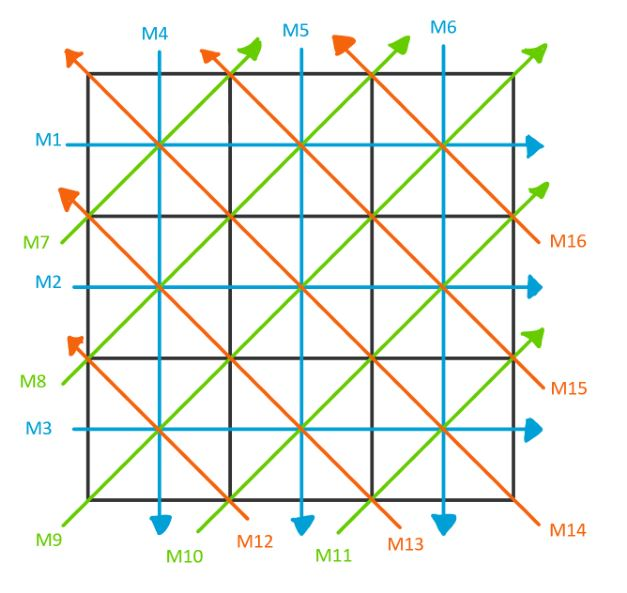
\includegraphics{plots/Projektionen.JPG}
  \caption{Mögliche Durchstrahlungsrichtungen durch die aus Elementarwürfeln bestehende Probe.}
  \label{fig:Projektionen}
\end{figure}
Anschließend werden der Reihe nach das Aluminiumgehäuse, welches die Elementarwürfel zusammenhält, sowie ein Aluminium und ein Bleiwürfel in den Strahlengang gebracht um Referenzwerte für die Messung der unbekannten Materialkomposition zu bestimmen. Die Proben werden entlang der Richtungen M1, M2, M8 und M9 aus Abbildung \ref{fig:Projektionen} vermessen. Es wird in $Maestro$ eine Messzeit von 300s eingestellt.\\
Anschließend wird ein Würfel mit Unbekannter Zusammensetzung in den Strahlengang gebracht. Dieser wird bei einer Messzeit von 400s entlang der Richtungen ???? aus Abbildung \ref{fig:Projektionen} vermessen.
